\documentclass[11pt]{homework}

\usepackage{tikz}
\usetikzlibrary{arrows,shapes,calc,positioning}
\usepackage{courier}
\def\defaultHypSeparation{\hskip 0.1in}
\usepackage{listing}
\lstset{
	basicstyle=\footnotesize\ttfamily,
	numbers=left,
	stepnumber=1,
	mathescape=true	
}

\usepackage{multicol}

% TODO: replace these with your information
\newcommand{\hwname}{Chiao Hsieh}
\newcommand{\hwemail}{chsieh16@illinois.edu}
\newcommand{\hwtype}{Homework}
\newcommand{\hwnum}{II}
\newcommand{\hwclass}{CS 426: Compiler Construction}
\newcommand{\hwlecture}{}
\newcommand{\hwsection}{}

\renewcommand{\questiontype}{Problem}
\newcommand{\TT}{\ensuremath{\mathtt{true}}}
\newcommand{\FF}{\ensuremath{\mathtt{false}}}

\begin{document}
\maketitle

% Your content

\question
(\textit{50 points.}) Dominators, loops and reducibility:

\begin{enumerate}[label=(\alph*)]

\begin{multicols}{2}

\item Ans. CFG for function \verb|ugly|

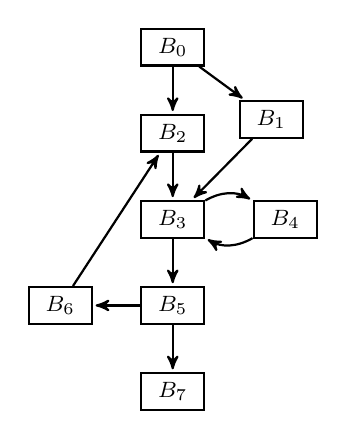
\begin{tikzpicture}[->,>=stealth',shorten >=1pt,auto,node
      distance=6mm,thick,
      every node/.style={rectangle,draw,minimum width=0.8cm, font=\footnotesize\ttfamily}]

    \node (B0) {$B_0$};
    \node[below right=of B0] (B1) {$B_1$};
    \node[below=of B0] (B2) {$B_2$};
    \node[below=of B2] (B3) {$B_3$};
    \node[right=of B3] (B4) {$B_4$};
    \node[below=of B3] (B5) {$B_5$};
    \node[left =of B5] (B6) {$B_6$};
    \node[below=of B5] (B7) {$B_7$};
	
	\path
        (B0) edge (B1)
        (B0) edge (B2)
        (B1) edge (B3)
        (B2) edge (B3)
        (B3) edge [bend left] (B4)
        (B3) edge (B5)
        (B4) edge [bend left] (B3)
        (B5) edge (B6)
        (B5) edge (B7)
        (B6) edge (B2)
	;
\end{tikzpicture}

\item Ans. Dominator Tree

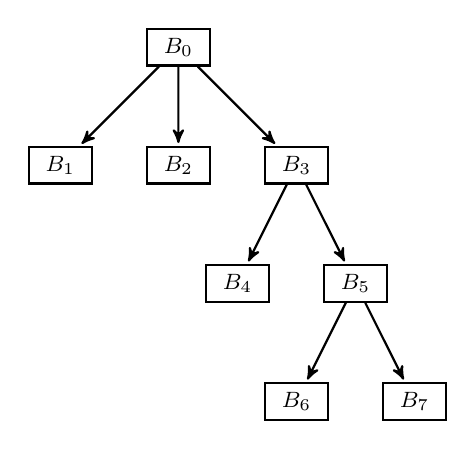
\begin{tikzpicture}[->,>=stealth',shorten >=1pt,auto,node
      distance=6mm,thick,
      every node/.style={rectangle,draw,minimum width=0.8cm, font=\footnotesize\ttfamily}]
	\node (B0) {$B_0$}
      child {node (B1) {$B_1$}}
      child {node (B2) {$B_2$}}
      child {node (B3) {$B_3$}
        child {node (B4) {$B_4$}}
        child {node (B5) {$B_5$}
          child {node (B6) {$B_6$}}
          child {node (B7) {$B_7$}}
        }
      };
\end{tikzpicture}

\end{multicols}

\item Ans. The set of back edges: $\{B_4\to B_3\}$

For edge $B_4\to B_3$, the natural loop is $\{B_3, B_4\}$

\item Ans. Following the definition of reducible flow graph,
every edge in the CFG should be a forward edge or a back edge.
However, edge $S_6 \to S_2$ is neither since $S_2$ doesn't dominate $S_6$.
Hence, the CFG is irreducible.

\item Ans. We modify the program by duplicating the body of $B_2$ after $B_6$,
and directly \texttt{goto} $B_3$.
\begin{lstlisting}[language=C]
void ugly(int N, int A[]) {
    int j = 0, *p, sum;         /* Basic block $B_0$ */
    if (N <= 1000)
        goto 10;                /* Basic block $B_1$ */
20: N = 1000;
    p = &W;                     /* Assume $W$ is a global */
10: for (i=0; i < N; i++)
        sum = sum + *p * A[i];
    j = j+1;
    if (j < N)
    {
        N = 1000;               /* Duplicate the body of $B_2$*/
        p = &W;
        goto 10;                /* Goto basic block $B_3$ */
    }
    printf("sum = %d\n", sum);
}
\end{lstlisting}

\end{enumerate}

\question

\begin{enumerate}[label=(\alph*)]

\item Ans.
\begin{multicols}{2}

\begin{center}
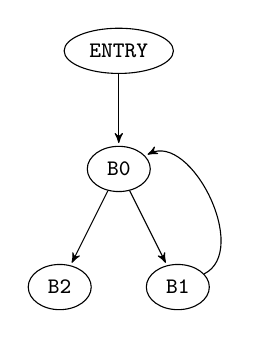
\begin{tikzpicture}[->,>=stealth',shorten >=1pt,auto,node
distance=6mm,
every node/.style={ellipse,draw,minimum width=0.8cm, font=\footnotesize\ttfamily}]

\node (entry) {ENTRY}
  child {node (B0) {B0}
    child {node (B2) {B2}}
    child {node (B1) {B1}}
  };

\path (B1) edge [bend right=90] (B0);

\end{tikzpicture}
\end{center}
\columnbreak

\begin{enumerate}[label=\roman*.]
\item 3 iterations
\item \texttt{ENTRY-B0-B1-B0-B2}
\item Assuming we want to propagate a definition $d$ in B1 to B2,
\begin{flushleft}
Iteration 1, $d$ will be in Out[B1].\\
Iteration 2, $d$ will be propagated to Out[B0] and Out[B2] by B1 $\to$ B0.\\
Iteration 3, nothing changes. End.
\end{flushleft}
\end{enumerate}
\columnbreak

\end{multicols}

\item Ans.

\begin{multicols}{2}

\centering
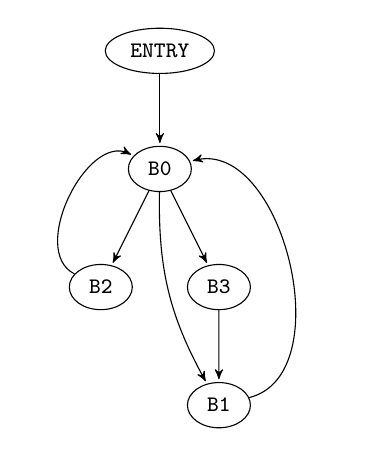
\begin{tikzpicture}[->,>=stealth',shorten >=1pt,auto,node
    distance=6mm,
    every node/.style={ellipse,draw,minimum width=0.8cm, font=\footnotesize\ttfamily}]
    
    \node (entry) {ENTRY}
    child {node (B0) {B0}
        child {node (B2) {B2}}
        child {node (B3) {B3}
            child {node (B1) {B1}}}
    };
    
    \path 
      (B0) edge [bend right=15] (B1)
      (B1) edge [bend right=90] (B0)
      (B2) edge [bend left=90] (B0);    
\end{tikzpicture}
    
\columnbreak
\begin{enumerate}[label=\roman*.]
    \item 3 iterations
    \item \texttt{ENTRY-B0-B1-B0-B2}
    \item Assuming we want to propagate a definition $d$ in B1 to B2,
    \begin{flushleft}
        Iteration 1, $d$ will be in Out[B1].\\
        Iteration 2, $d$ will be propagated to Out[B0] and Out[B2] by B1 $\to$ B0.\\
        Iteration 3, nothing changes. End.
    \end{flushleft}
\end{enumerate}
\end{multicols}    

\item Ans.

\begin{multicols}{2}
    \centering
    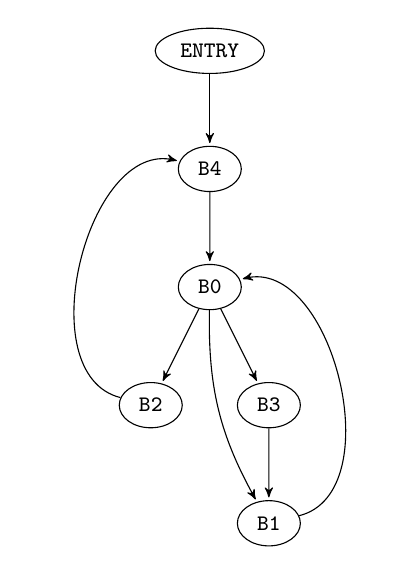
\begin{tikzpicture}[->,>=stealth',shorten >=1pt,auto,node
    distance=6mm,
    every node/.style={ellipse,draw,minimum width=0.8cm, font=\footnotesize\ttfamily}]
    
    \node (entry) {ENTRY}
    child {node (B4) {B4}
        child {node (B0) {B0}
            child {node (B2) {B2}}
            child {node (B3) {B3}
                child {node (B1) {B1}}}}
    };
    
    \path 
    (B0) edge [bend right=15] (B1)
    (B1) edge [bend right=90] (B0)
    (B2) edge [bend left=90] (B4);    
    \end{tikzpicture}
    
    \columnbreak
    \begin{enumerate}[label=\roman*.]
        \item 4 iterations
        \item \texttt{ENTRY-B4-B0-B1-B0-B2-B4}
        \item Assuming we want to propagate a definition $d$ in B1 to B4,
        \begin{flushleft}
            Iteration 1, $d$ will be in Out[B1].\\
            Iteration 2, $d$ will be propagated to Out[B0] and Out[B2] by B1 $\to$ B0.\\
            Iteration 3, $d$ will be propagated to Out[B4] by B2 $\to$ B4.\\
            Iteration 4, nothing changes. End.
        \end{flushleft}
    \end{enumerate}
\end{multicols}

\item Ans.

\begin{multicols}{2}
    \centering
    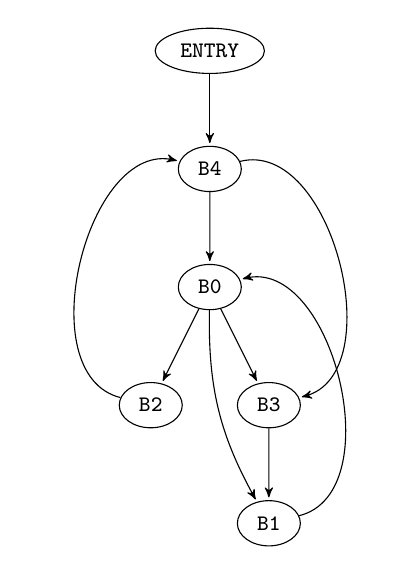
\begin{tikzpicture}[->,>=stealth',shorten >=1pt,auto,node
    distance=6mm,
    every node/.style={ellipse,draw,minimum width=0.8cm, font=\footnotesize\ttfamily}]
    
    \node (entry) {ENTRY}
    child {node (B4) {B4}
        child {node (B0) {B0}
            child {node (B2) {B2}}
            child {node (B3) {B3}
                child {node (B1) {B1}}}}
    };
    
    \path 
    (B0) edge [bend right=15] (B1)
    (B1) edge [bend right=90] (B0)
    (B2) edge [bend left=90] (B4)
    (B4) edge [bend left=90] (B3);    
    \end{tikzpicture}
    
    \columnbreak
    \begin{enumerate}[label=\roman*.]
        \item 4 iterations
        \item \texttt{ENTRY-B4-B0-B1-B0-B2-B4}
        \item Assuming we want to propagate a definition $d$ in B1 to B4,
        \begin{flushleft}
            Iteration 1, $d$ will be in Out[B1].\\
            Iteration 2, $d$ will be propagated to Out[B0] and Out[B2] by B1 $\to$ B0.\\
            Iteration 3, $d$ will be propagated to Out[B4] by B2 $\to$ B4.\\
            Iteration 4, nothing changes. End.
        \end{flushleft}
    \end{enumerate}
\end{multicols}

\end{enumerate}

\question
Ans.

Gen[$B_2$] = \{$D_{Y_3}, D_{Z_3}, D_{X_4}, D_{N_5}$\}

Gen[$B_3$] = \{$D_{X_1}, D_{N_2}$\}

Kill[$B_2$] = \{$D_{X_1}, D_{X_7}, D_{X_8}, D_{N_2}, D_{N_{11}}, D_{N_{12}} $\}

Kill[$B_3$] = \{$D_{X_4}, D_{X_7}, D_{X_8}, D_{N_5}, D_{N_{11}}, D_{N_{12}} $\}

\question
Ans.

\textbf{{
\begin{tabular}[h]{|r|c|c|c|c|l|}
	\hline
	                                 & SCCP & DCE & GCSE & EXPR & Simplest Sequence Needed \\ \hline
	$\mathbf{x}_2$  is dead          & No   & Yes & No   & No   & DCE                      \\
	$\mathbf{c}_6 = \mathbf{i}_3$    & Yes  & No  & No   & No   & SCCP                     \\
	$\mathbf{j}_7 = \mathbf{c}_6$    & Yes  & No  & No   & No   & SCCP                     \\
	$\mathbf{idx}_{17} = \mathbf{k}$ & No   & No  & Yes  & No   & GCSE                     \\
	$\mathbf{d}_{18} = 0$            & No   & No  & No   & Yes  & GCSE; EXPR \\
	$\mathbf{i}_{10} = 13$           & Yes  & No  & No   & No   & GCSE; EXPR; SCCP \\ \hline
\end{tabular}
}}

\question
\begin{enumerate}[label=(\alph*)]
\item Ans.

$in[B] = \bigcap\limits_{p : p \to B} out[p]$,
where $p \to B$ means $p$ is a predecessor block of $B$.

$out[B] = (in[B] \cup e\_gen[B]) \setminus e\_kill[B]$

\item Ans.

Under this setting, we assume initially every expression is available at every
basic block except for entry block.
The reason is that an available expression may not be generated by all
predecessors of a given current block.
It can be generated by the dominator of current block
while the expression is not killed during every path to current block.
If we initialized with only $e\_gen[B]$, we can not capture this kind of
available expressions since the expression is not generated by all predecessors
and will be removed by intersection.

\end{enumerate}

\question
\begin{enumerate}[label=(\alph*)]

\item Ans.

For ``local'' dataflow variables of a given basic block $B$, we denote the set of variables definitely initialized by instructions in $B$ as $gen[B]$.
This can be computed locally in a basic block since we only include all variables appeared at LHS of an assignment.
However, if the LHS is a deference of a pointer, we will have to do the points-to analysis first.
If the pointer is proven to point to only one variable $v$,
then $v$ will be included in $gen[B]$.
Otherwise, $v$ will not be included.

\item Ans.

$InitSafe\_in[B] = \bigcap\limits_{p:p \to B} InitSafe\_out[p]$. \quad Get variables initialized in all predecessors.

$InitSafe\_out[B] = InitSafe\_in[B] \cup gen[B]$ \quad Add variables assigned in $B$ as initialized.

Based on the definition, we know that $InitSafe\_in[B]$ is non-increasing and monotonic
since intersection does not add more elements.
Similarly, $InitSafe\_out[B]$ is monotonic because $gen[B]$ is constant.

\item Ans.

Initially,\\
$InitSafe\_out[s]= gen[s]$\\
$InitSafe\_out[B] = U$ for all other basic blocks $B$ where $U$ is all variables in the procedure.
We don't care about initial values of $InitSafe\_in$ because it will be overwritten at first iteration.  

The order to visit basic blocks won't affect the final result but the number of iterations to converge.
We choose the same as the one in lecture slides, that is, propagating through acyclic paths,
so we can guarantee the upper bound of the number of iterations.

\pagebreak

\item Ans. Stop at second iteration since $out_1 = out_2$

\newcommand{\EMP}{\emptyset}
$$
\begin{array}{l||l|l||l|l||l|l}
	    & gen & out_0     & in_1 & out_1     & in_2 & out_2     \\
	B_0 & j   & j         &      & j         &      & j         \\
	B_1 &     & j, p, sum & j    & j         & j    & j         \\
	B_2 & p   & j, p, sum & j    & j, p      & j    & j, p      \\
	B_3 & i   & j, p, sum & j    & j, i      & j    & j, i      \\
	B_4 & sum & j, p, sum & j, i & j, i, sum & j, i & j, i, sum \\
	B_5 & j   & j, p, sum & j, i & j, i      & j, i & j, i      \\
	B_6 &     & j, p, sum & j, i & j, i      & j, i & j, i      \\
	B_7 &     & j, p, sum & j, i & j, i      & j, i & j, i
\end{array}
$$
\end{enumerate}

\end{document}